\documentclass[10pt]{beamer}
\usepackage[slovak]{babel}
\usetheme{metropolis}
\usepackage{amsthm}
\usepackage{appendixnumberbeamer}
\usepackage{booktabs}
\usepackage[scale=2]{ccicons}
\usepackage{pgfplots}
\usepgfplotslibrary{dateplot}
\usepackage{xspace}
\addtobeamertemplate{block begin}{}{\vspace{0.5pt}}
\addtobeamertemplate{alertblock begin}{}{\vspace{2pt}}
%\addtobeamertemplate{block end}{}{\vpspace{1pt}}
\newcommand{\themename}{\textbf{\textsc{metropolis}}\xspace}



\title{Porovnanie niekoľkých typov rekurentných neurónových sietí z hľadiska hĺbky pamäte}
\subtitle{Diplomová práca}
% \date{\today}
\date{}
\author{Jaroslav Ištok}
\institute{Školiteľ: doc. RNDr. Martin Takáč, PhD.}
% \titlegraphic{\hfill\includegraphics[height=1.5cm]{logo.pdf}}

\begin{document}

\maketitle

\begin{frame}{Obsah}
  \setbeamertemplate{section in toc}[sections numbered]
  \tableofcontents
\end{frame}


\section{Rekurentné neurónové siete}

\begin{frame}[fragile]{Rekurentné neurónove siete}
  \begin{itemize}
    \item Pracujú s určitým druhom historického kontextu
    \item Kontext je tvorený minulými stavmi a vstupmi siete a predstavuje formu pamäťe.
    \item Výstup siete je ovplyvnený aj minulými vstupmi a nie iba aktuálnym
    \item Rekurentné SOM (RecSOM a MSOM)
    \item SRN s Elmanovou architektúrou 
  \end{itemize}
\end{frame}

\begin{frame}[fragile]{Pamäťová hĺbka rekurentnej neurónovej siete}
  \begin{block}{Pamäťová hĺbka - definícia}
    Hĺbka pamäti neurónovej siete vyjadruje dĺžku historického kontextu, ktorý má 
    ešte vplyv na aktuálny výstup siete. Ak je hĺbka pamäti $N$, vstupy v čase väčšom ako 
    $(T - N)$ nemajú vplyv na výstup v čase $T$.
  \end{block}
\end{frame}


\section{Úvod do SOM}
\begin{frame}[fragile]{SOM}
  \begin{itemize}
    \item učenie bez učiteľa
    \item zhlukovanie dát
    \item zachovanie topologických vlastností dát
  \end{itemize}

  Hľadanie víťaza
  \begin{equation*}
    i^* = argmin_i||x-w_i|| 
  \end{equation*}

  Aktualizácia váh
  \begin{equation*}
    w_i(t + 1) = w_i(t) + \alpha(t)h(i^*, i)[x(t) - w_i(t)]
  \end{equation*}
\end{frame}

\begin{frame}[fragile]{Rekurentná SOM}
  \begin{itemize}
    \item rozšírená o kontext
    \item pridané kontextové váhy
  \end{itemize}
  
  Výpočet vzdialenosti
  \begin{equation*} 
    d_i = (1 - \alpha) \cdot ||x(t) - w_i||^{2} + \alpha \cdot ||y(t-1) - c_i||^{2} 
  \end{equation*}

  Aktualizácia váh
  \begin{equation*}
    w_i(t + 1) = w_i(t) + \alpha(t)h(i^*, i)[x(t) - w_i(t)]
  \end{equation*}

  Aktualizácia kontextových váh
  \begin{equation*}
    c_i(t + 1) = c_i(t) + \alpha(t)h(i^*, i)[y(t - 1) - c_i(t)]
  \end{equation*}
\end{frame}

\begin{frame}[fragile]{Pamäťová hĺbka v rekurentnej SOM}

  \begin{block}{Spôsob určovania pamäťovej hĺbky v rekurentných SOM}
    Každý neurón má navyše pamäťové okno, do ktorého sú ukladané vstupy, pre ktoré bol daný neurón víťazom.
    Neukladáme však iba vstupy, ale vždy $k$ posledných vstupov, kde $k$ je veľkosť posuvného okna na vstupnej sekvencii.
  \end{block}

  \begin{block}{Pamäťová hĺbka v rekurentných SOM}
    Vážený priemer dĺžok najdlhších spoločných podpostupností reťazcov (určovaných od konca) v pamäťových oknách všetkých neurónov v sieti.
    Priemer je váhovaný počtom reťazcov uložených v jednotlivých pamäťových oknách.
    
  \end{block}

  \begin{block}{Pamäťová hĺbka v rekurentných SOM}
    Čiže napríklad ak by pamäťové okno obsahovalo \uv{abbda\textbf{bb}} a \uv{bbbac\textbf{bb}}, potom pamäťová hĺbka pre toto okno bude \textbf{2}
  \end{block}
\end{frame}

\section{Experiment so SOM}
\begin{frame}[fragile]{Experiment so SOM}

  \begin{block}{Čo bolo cieľom experimentu?}
    Nájsť optimálne hodnoty parametrov, pri ktorých daný typ siete dosahuje
    najvyššiu hodnotu pamäťovej hĺbky a porovnať siete s optimálnymi parametrami.
  \end{block}

\end{frame}



\begin{frame}[fragile]{Priebeh experimentu}

  \begin{itemize}
    \item Siete sme natrénovali s rôznymi kombináciami parametrov, ktoré ovplyvňujú váhu kontextu vo výpočte vzdialenosti a zloženie samotného kontextu.
    \item Použili sme postupne zmenšujúcu sa gausovskú funkciu susednosti
    \item Postupne klesajúca rýchlosť učenia
    \item Ako trénovacie dáta sme použili náhodne vygenerovanú postupnosť písmen \textbf{abcd}
    \item Na záver sme porovnali pamäťové hĺbky sietí s optimálnymi parametrami
    \item Vstupmi su 1-hot enkódované písmená
  \end{itemize} 

  Použitá funkcia susednosti
  \begin{equation}
		N(i^{*}, i) = \exp^{- \frac{d^{2}_{E}(i^{*}, i)}{\lambda^{2}(t)}}
	\end{equation}

\end{frame}

\subsection{RecSOM}
\begin{frame}[fragile]{RecSOM}

  \begin{block}{RecSOM kontext, vzdialenosť a parametre}
    
    \begin{equation*}
      y(t) = [y_1(t-1), ..., y_{N}(t-1)]  \quad c, r \in R^{N}
    \end{equation*}
    \begin{equation*}
      y_i = \exp(-d_i)
    \end{equation*}
    \begin{equation*}
      d_i = (1 - \alpha) \cdot ||x(t) - w_i||^{2} + \alpha \cdot ||y(t-1) - c_i||^{2} \quad c_{i} \in R^{N}
    \end{equation*}

    Pri RecSOM máme iba parameter $\alpha$
    
  \end{block}

  \begin{table}[h!]
    \centering
    \begin{tabular}{|c|c|} 
     \hline
     Parameter & Hodnota \\ 
     \hline\hline
     Hodnoty alpha & 0 - 1  (krok: 0.01) \\ 
     \hline
     Rozmer & 30x30  \\
     \hline
     Počet epôch trénovania & 20 \\
     \hline
     Veľkosť posuvného okna & 10  \\
     \hline
    \end{tabular}
    \caption{Trénovacie parametre RecSOM siete}
    \end{table}

\end{frame}
\begin{frame}[fragile]{RecSOM výsledky}
 \begin{figure}[H]
  \centering
  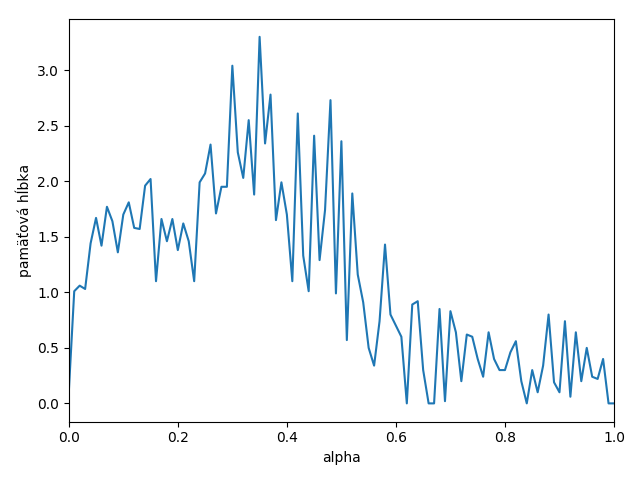
\includegraphics[width=0.49\textwidth]{assets/r_memory_span}
  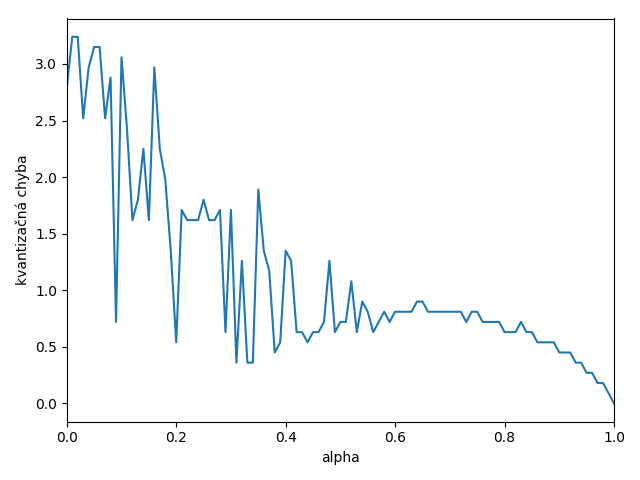
\includegraphics[width=0.49\textwidth]{assets/r_errors}
  \caption{Výsledky RecSOM}
\end{figure}

\end{frame}

\subsection{Activity RecSOM}
\begin{frame}[fragile]{Activity RecSOM}

  \begin{block}{Activity RecSOM}
    Pri RecSOM sme chceli sme ovplyvniť
    spôsob výpočtu kontextu. Preto sme pozmenili spôsob výpočtu aktivácie.
    Pridalo nám to ďaľší parameter $\beta$.
    \begin{equation*}
      y_{i} = \exp^{(-\beta \cdot d_{i}^2)}
    \end{equation*}
  \end{block}

  \begin{figure}[H]
    \centering
    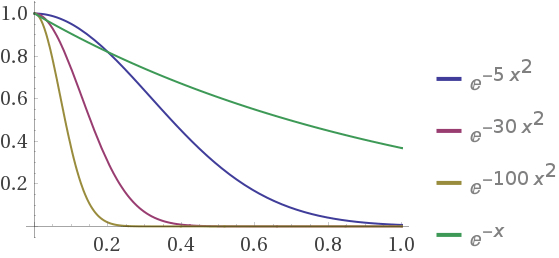
\includegraphics[width=\textwidth]{assets/plots}
    \caption{Grafy priebehu funkcií na výpočet aktivácií neurónov v Activity RecSOM}
\end{figure}

\end{frame}

\begin{frame}[fragile]{Activity RecSOM}
\begin{table}[h!]
  \centering
  \begin{tabular}{|c|c|} 
   \hline
   Parameter & Hodnota \\ 
   \hline\hline
   Hodnoty alpha & 0 - 1 (krok 0.1) \\ 
   \hline
   Hodnoty beta & [5.0,12.0,13.0,14.0,15.0,20.0,30.0,40.0,50.0,100.0]\\ 
   \hline
   Veľkosť & 30x30  \\
   \hline
   počet epôch trénovania & 20  \\
   \hline
   veľkosť posuvného okna & 10  \\
   \hline
  \end{tabular}
  \caption{Parametre Activity RecSOM siete}
\end{table}
\end{frame}

\begin{frame}[fragile]{Activity RecSOM výsledky}

  % heatmapu hlbok a chyb
  \begin{figure}[H]
   \centering
   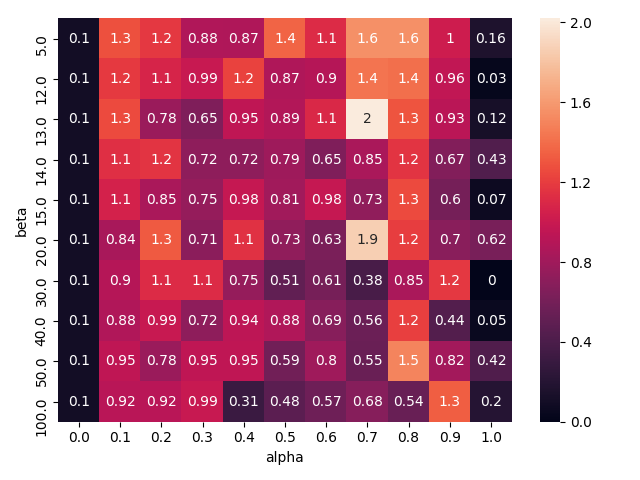
\includegraphics[width=0.49\textwidth]{assets/ar_memory_span}
   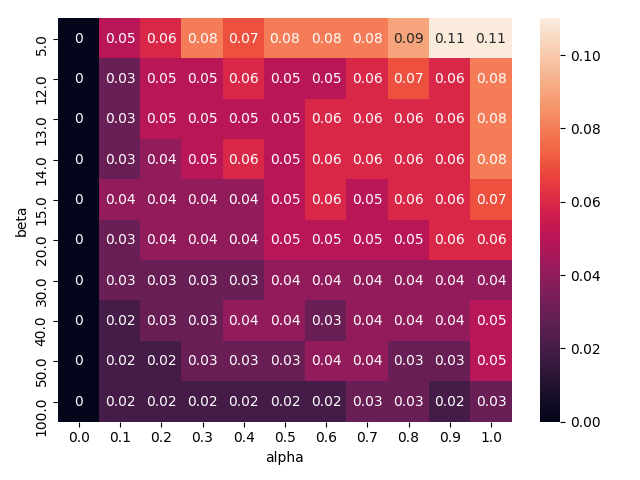
\includegraphics[width=0.49\textwidth]{assets/ar_errors}
   \caption{Výsledky Activity RecSOM}
 \end{figure}


\end{frame}

\subsection{MSOM}
\begin{frame}[fragile]{Merge SOM}

  \begin{block}{MSOM kontext, vzdialenosť a parametre}
    
    \begin{equation}
      y(t) = (1 - \beta) \cdot w_{i^{*}}(t-1) + \beta \cdot c_{i^{*}}(t-1)
    \end{equation}
    \begin{equation*}
      d_i = (1 - \alpha) \cdot ||x(t) - w_i||^{2} + \alpha \cdot ||y(t-1) - c_i||^{2} \quad c_{i} \in R^{N}
    \end{equation*}

    Pri MSOM máme parametere $\alpha$ a $\beta$

  \end{block}

    \begin{table}[h!]
      \centering
      \begin{tabular}{|c|c|} 
       \hline
       Parameter & Hodnota \\ 
       \hline\hline
       Hodnoty alpha & 0 - 1 (krok 0.1)  \\ 
       \hline
       Hodnoty beta & 0 - 1  (krok 0.1) \\ 
       \hline
       Veľkosť & 30x30  \\
       \hline
       Počet epôch & 20  \\
       \hline
       Veľkosť posuvného okna & 10  \\
       \hline
      \end{tabular}
      \caption{Parametre MSOM siete}
    \end{table}
  
\end{frame}
\begin{frame}[fragile]{MSOM výsledky}

  % heatmapu hlbok a chyb
  \begin{figure}[H]
   \centering
   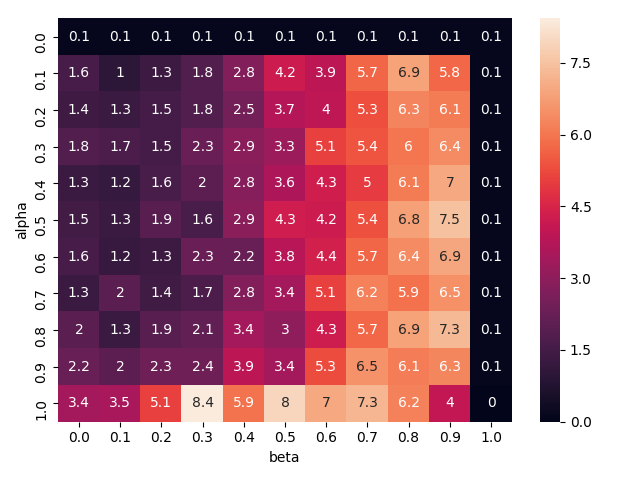
\includegraphics[width=0.49\textwidth]{assets/m_memory_span}
   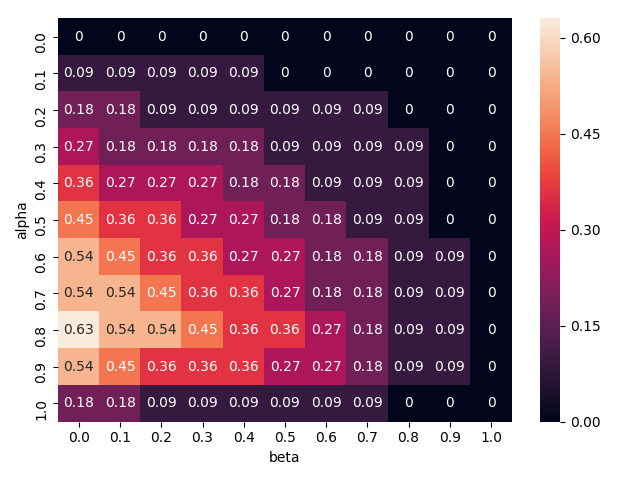
\includegraphics[width=0.49\textwidth]{assets/m_errors}
   \caption{Výsledky MSOM}
 \end{figure}


\end{frame}

% decay msom
\subsection{Decay MSOM}
\begin{frame}[fragile]{Decay MSOM}

  \begin{block}{Decay MSOM kontext, vzdialenosť a parametre}
    
    \begin{equation} 
      c_{t} = x_{t} + \beta * c_{t-1}
    \end{equation}
    \begin{equation}
      c = \beta^{0} \cdot x_{t} + \beta^{1} \cdot x_{t-1} + 
      \beta^{2} \cdot x_{t-2} \ddots \beta^{n} \cdot x_{t-n}
    \end{equation}

    Modifikovaná verzia MSOM, kde sme chceli vyskúšať odlišný druh 
    kontextu, ktorý nie je tvorený minulými stavmi siete ale samotnou históriou vstupov siete.
    Pri Decay MSOM máme parametre $\alpha$ a $\beta$
  \end{block}
    \begin{table}[h!]
      \centering
      \begin{tabular}{|c|c|} 
       \hline
       Parameter & Hodnota \\ 
       \hline\hline
       Hodnoty alpha & 0 - 1 (krok 0.1)  \\ 
       \hline
       Hodnoty beta & 0 - 1  (krok 0.1) \\ 
       \hline
       Veľkosť & 30x30  \\
       \hline
       Počet epôch trénovania & 20  \\
       \hline
       Veľkosť posuvného okna & 10 \\
       \hline
      \end{tabular}
      \caption{Parametre Decaying MSOM siete}
    \end{table}
\end{frame}
\begin{frame}[fragile]{Decay MSOM výsledky}

  % heatmapu hlbok a chyb
  \begin{figure}[H]
   \centering
   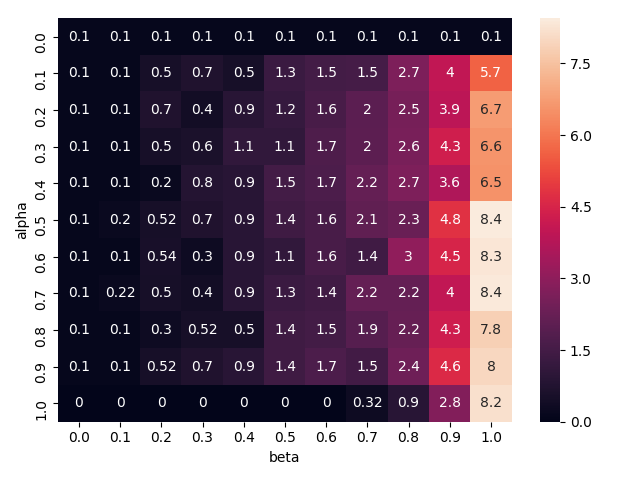
\includegraphics[width=0.49\textwidth]{assets/dm_memory_span}
   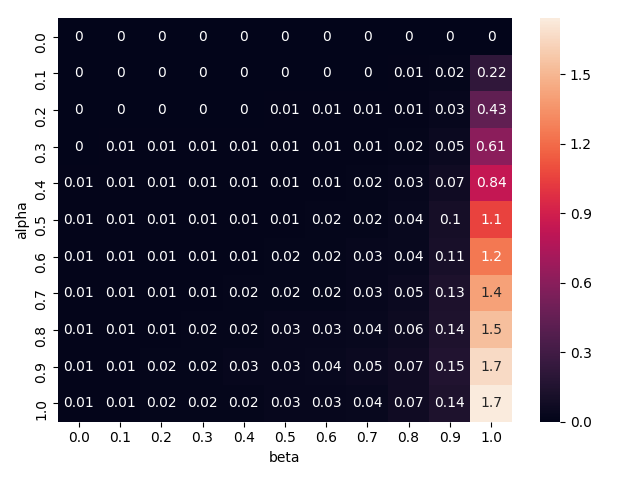
\includegraphics[width=0.49\textwidth]{assets/dm_errors}
   \caption{Výsledky Decay MSOM}
 \end{figure}


\end{frame}

\begin{frame}[fragile]{Vyhodnotenie výsledkov experimentu so SOM}
  \begin{itemize}
    \item Problém s rozdielom v dimenziách medzi váhovými a kontextovými vektormi pri RecSOM a Activity RecSOM
    \item Vplyv zloženia kontextu na pamäťovú hĺbku
    \item DecaySOM
    \item Výpočtová náročnosť RecSOM vs MSOM
  \end{itemize}
\end{frame}

\section{Úvod do SRN}

\begin{frame}[fragile]{SRN s Elmanovou architektúrou}
  \begin{itemize}
    \item Trénovanie pomocou BPTT
    \item Skrytá vrstva 
    \item Stavový priestor na skrytej vrstve
  \end{itemize}

  \begin{figure}[H]
    \centering
    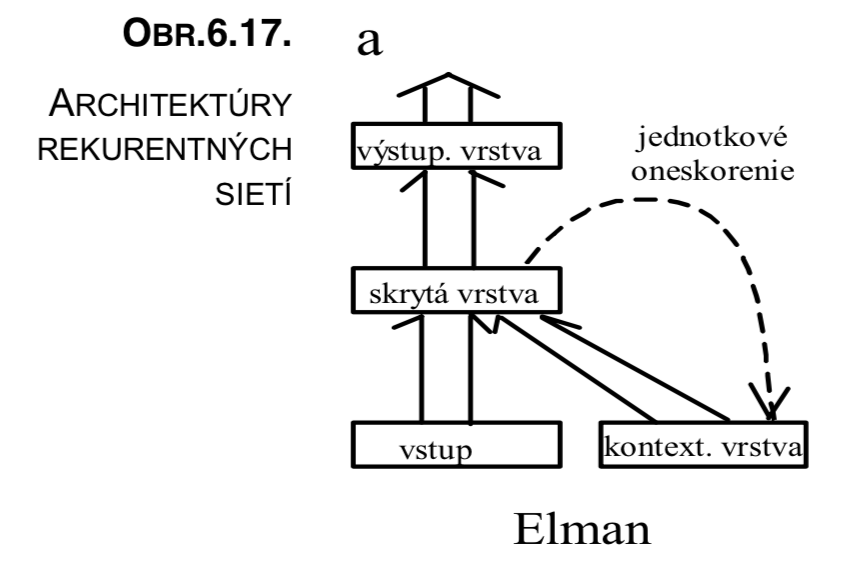
\includegraphics[width=6cm]{assets/elman_architecture}
    \caption{Architektúra Elmanovej siete}
  \end{figure}
\end{frame}

\section{Experiment s SRN}

\begin{frame}[fragile]{Experiment s SRN}
  \begin{itemize}
    \item Hľadanie spôsobu merania pamäťovej hĺbky
    \item Analýza stavového priestoru
    \item Dendrogram
  \end{itemize}

  \begin{table}[h!]
    \centering
    \begin{tabular}{|c|c|} 
    \hline
    Parameter & Hodnota \\ 
    \hline
    veľkosť skrytej vrstvy & 30  \\
    \hline
    počet epôch & 100  \\
    \hline
    počet krokov do minulosti (T) & 5 \\
    \hline
    \end{tabular}
    \caption{Trénovacie parametre SRN s Elmanovou architektúrou}
    \label{table:1}
\end{table}

\end{frame}

\begin{frame}[fragile]{Dendrogram}
\begin{figure}[H]
  \centering
  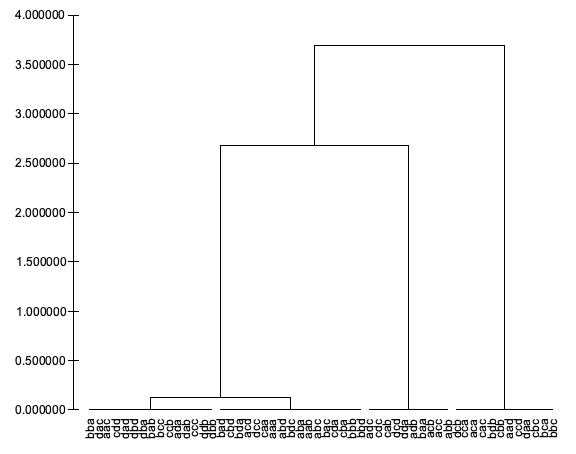
\includegraphics[width=8cm]{assets/dendrogram}
  \caption{Dendrogram pre Elmanovu sieť}
  \label{dendrogram}
\end{figure}
\end{frame}

\section{Otázky}
\begin{frame}{Otázky školiteľ}
  
  \begin{block}{Otázka}
    Podrobne popíšte, ako by ste použitím PCA vizualizovali v 2D na ktoré časti skrytého priestoru sa zobrazujú jednotlivé vstupné sekvencie a čo by vám to mohlo napovedať o hĺbke pamäti SRN
  \end{block}  

\end{frame}


\begin{frame}{Otázky školiteľ}
  \begin{block}{1. Odpoveď}
    Skrytý priestor v SRN je vysoko rozmerný, čiže vstupy sú akokeby zobrazované do vysoko rozmerného stavového priestoru na skrytej vrstve siete.  
    Každý vstup spôsobý nejakú aktiváciu neurónov na skrytej vrstve a toto je jeden bod v tom priestore.
    Keďže body vo vysokorozmernom priestore si nevieme vizualizovať, môžeme zredukovať ich dimenzie, napríklad pomocou PCA. 
    Keď potom vezmeme napríklad prvé dva principiálne komponenty a vykreslíme 2D scatter graf (projekciu do roviny) z týchto komponentov, tak sa nám vytvoria skupiny, kde každá skupina predstavuje vstupy, ktoré majú nejakú spoločnú vlastnosť.
    O pamäťovej hĺbke nám to moc nepovie, resp. sú to len 2D projekcie z veľarozmerného priestoru a nepredsatvujú skutočnú blízkosť vstupov v priestore.
    Dendrogram nám môže o pamäťovej hĺbke povedať viac, kedže ten reprezentuje skutočné vzdialenosti jednotlivých bodov v priestore.
  \end{block}  
\end{frame}
  


\begin{frame}{Otázky školiteľ}
  \begin{block}{2. otázka}
    2. V časti 5.7 spomínate, že Activity RecSOM by sa dala upraviť tak, že by vracala iba Gausovskú aktivitu okolo víťaza. Ako by ste ju upravili? Očakávate, že by takto upravená RecSOM dávala z hľadiska hĺbky pamäti výsledky podobnejšie na štandardnú RecSOM, alebo na MSOM? Prečo?
  \end{block}
\end{frame}

\begin{frame}{Otázky školiteľ}
  \begin{block}{2. odpoveď}
    Vzorec by som ponechal tak ako je pri Activity RecSOM, 
    teda gaussian s parametrom $\beta$ ktorým vieme ovplyvňovať strmosť (priebeh) tejto funkcie.
    Zmenila by sa hodnota vzdialenosti $d$. 
    Namiesto súčtu euklidovských vzdialeností, by sme použili vzdialenosť 
    daného neurónu od víťazného neurónu v mape (podobne ako pri funkcii susednosti), 
    a aktivita zvyšných neurónov by závisela od ich vzdialenosti od víťazného neurónu v samotnej mape a nie vzdialenosti vo vektorovom priestore. 
    Aktivita by nebola priamo ovplyvnená stavmi siete, ale iba samotnou pozíciou neurónu vzhľadom na víťazný neurón v danom kroku. 

    Podľa mňa budú výsledky takejto siete podobné výsledkom obyčajnej RecSOM čo sa týka hĺbky pamäte, 
    pretože kontext neobsahuje vlastnosti víťaza (ktoré sa ukázali ako dôležité z hľadiska hĺbky pamäte).
    
 

  \end{block}
\end{frame}

\begin{frame}{Otázky oponent}
  
  \begin{block}{1.Otázka}
    Pripraviť porovnanie kvality predikcie pre výsledky zo str. 43 až 47 plus kvalitu predikcie pre 3 trénovacie sety pre Elmanovu SRN. 
  \end{block}

  \begin{block}{2.Otázka}
    Ako hĺbka pamäte súvisí s kvalitou predikcie? Je medzi nimi lineárny vzťah? Čiže čím väčšia hĺbka pamäte, tým lepšia predikcia? Dá sa to alebo nedá doložiť aj údajmi z literatúry?
  \end{block}


\end{frame}

\begin{frame}{Otázky oponent}

  \begin{block}{1.Odpoveď } 
    Pri našich implementáciach SOM nemáme žiadne predikcie (unsupervised model).
    Kvalitu organizácie nám reprezentuje kvantizačná chyba, ktorú sme merali a aj porovnávali s pamäťovou hĺbkou.

  \end{block}

  \begin{block}{2.Odpoveď}
    Neviem to porovnať, kedže sme nenašli (neimplementovali) spôsob na odmeranie hĺbky pamäte SRN.
    Ako chybovú funkciu používame log loss, ktorá počas trénovania klesala až po veľmi nízke hodnoty. Bohužiaľ to nemôžem porovnať s pamäťovou hĺbkou.
  \end{block}


\end{frame}



{\setbeamercolor{palette primary}{fg=black, bg=yellow}
\begin{frame}[standout]
  Ďakujem za pozornosť
\end{frame}
}

\appendix



\end{document}
